\newcommand{\expression}{\int\frac{4x^2}{\sqrt{529-4x^2}}dx}
\newcommand{\x}{\frac{23}{2}Sen\theta}
\newcommand{\dx}{\frac{23}{2}Cos\theta}
\newcommand{\denominator}{\sqrt{529-4\left(\x\right)^2}}
\newcommand{\numerator}{\frac{529\cdot23}{2}Sen^2\theta Cos\theta}
\newcommand{\identity}{\frac{1-Cos(2\theta)}{2}}

\textbf{Temática 4 - Sustitución trigonométrica}
\[\expression\]
\[
    \begin{aligned}
        a=\sqrt{529} && v=\sqrt{4x^2} \\
        a=23 && v=2x
    \end{aligned}
\]
\[v=aSen\theta\]
\[2x=23Sen\theta\]
\[x=\x\]
\[dx=\dx d\theta\]
\[\expression=\int\frac{4\left(\x\right)^2\dx}{\denominator}d\theta\]
\[\expression=\int\frac{\cancel{4}\left(\frac{529}{\cancel{4}}Sen^2\theta\right)\dx}{\denominator}d\theta\]
\[\expression=\int\frac{\numerator}{\denominator}d\theta\]
\[\expression=\int\frac{\numerator}{\sqrt{529-\cancel{4}\left(\frac{529}{\cancel{4}}Sen^2\theta\right)}}d\theta\]
\[\expression=\int\frac{\numerator}{\sqrt{529-529Sen^2\theta}}d\theta\]
\[\expression=\int\frac{\numerator}{\sqrt{529(1-Sen^2\theta)}}d\theta\]
\[\expression=\int\frac{\numerator}{\sqrt{529Cos^2\theta}}d\theta\]
\[\expression=\int\frac{\frac{529\cdot\cancel{23}}{2}Sen^2\cancel{\theta Cos\theta}}{\cancel{23Cos\theta}}d\theta\]
\[\expression=\int\frac{529}{2}Sen^2d\theta\]
\[
    \begin{aligned}
        Usamos && la && identidad && Sin^2\theta=\identity
    \end{aligned}
\]
\[\expression=\int\frac{529}{2}\cdot\identity d\theta=\frac{529}{4}\int(1-Cos(2\theta))d\theta\]
\[\expression=\frac{529}{4}\left(\theta-\frac{Sen(2\theta)}{2}\right)+C\]
\[x=\frac{23}{2}Sen\theta\]
\[Sen\theta=\frac{2x}{23}\]
\[\theta=Arcsen\left(\frac{2x}{23}\right)\]
\[\expression=\frac{529}{4}\left(Arcsin\left(\frac{2x}{23}\right)-\frac{2x}{23}\sqrt{1-\left(\frac{2x}{23}\right)^2}\right) + C
\]

\begin{figure}[h]
    \begin{center}
        \fbox{
            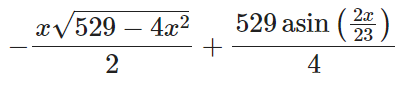
\includegraphics{comp-task4.png}
        }
        \caption{Integración por sustitución trigonométrica sympy}
    \end{center}
\end{figure}